%
% Wellengleichung
%
\section{Wellengleichung}
\kopfrechts{Wellengleichung}
Die Wellengleichung beschreibt die Fortpflanzung einer Welle
in einem elastischen Medium.
\index{Wellengleichung}%
In diesem Abschnitt wird die Wellengleichung im eindimensionalen
Fall hergeleitet.
Es stellt sich heraus, dass man sie als die Kontinuitätsgleichung
für die Impulsdichte und den Impulsstrom verstehen kann.

%
% Die Bewegung einer Saite
%
\subsection{Die Bewegung einer Saite}
%
% fig-saite.tex
%
% (c) 2025 Prof Dr Andreas Müller
%
\begin{figure}
\centering
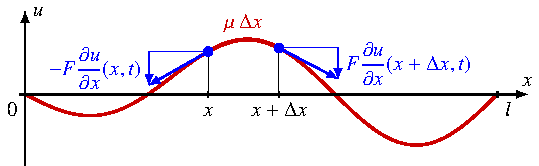
\includegraphics{chapters/080-feldgleichungen/images/saite.pdf}
\caption{Herleitung der eindimensionalen Wellengleichung für eine
schwingende Saite.
Auf das Segment der Masse $\mu\,\Delta x$ zwischen den Punkten $x$ und
$\Delta x$ wirkt eine resultierende Querkraft, die aus den blauen
Vektoren berechnet werden kann.
\label{buch:feldgleichungen:wellengleichung:fig:saite}}
\end{figure}
%
Wir betrachten eine Saite mit der linearen Massedichte $\mu$, die
zwischen den Punkten $0$ und $l$ entlang einer Geraden eingespannt
ist.
Die Spannung der Saite entlang der Geraden ist die Kraft $F$.
\index{Spannung}%
Die Funktion
\[
u
\colon
[0,l]\times \mathbb{R}
\to
\mathbb{R}
:
(x,t)
\mapsto
u(x,t)
\]
beschreibt die Auslenkung der Saite aus der Ruhelage in Abhängigkeit
von Position $x\in[0,l]|$ und der Zeit $t$.
\index{Auslenkung}%
\index{Ruhelage}%

Wir betrachten jetzt in kurzes Segment der Länge $\Delta x$ der Saite
zwischen den Koordinaten $x$ und $x+\Delta x$.
Die Masse dieses Segmentes ist $\mu \Delta x$.
Die Spannung der Saite übt eine Kraft auf das Segment aus.
Die Komponente in $x$-Richtung verschwindet.
Die Komponenten senkrecht zur Achse an den beiden 
Enden des Segmentes sind
\[
-F\frac{\partial u}{\partial x}(x,t)
\qquad\text{und}\qquad
F\frac{\partial u}{\partial x}(x+\Delta x,t),
\]
es wirkt also die gesamte Kraft
\[
F
\biggl(
\frac{\partial u}{\partial x}(x+\Delta x,t)
-
\frac{\partial u}{\partial x}(x,t)
\biggr).
\]
Das newtonsche Gesetz $F=ma$ besagt dann, dass
\index{newtonsches Gesetz}%
\[
F
\biggl(
\frac{\partial u}{\partial x}(x+\Delta x,t)
-
\frac{\partial u}{\partial x}(x,t)
\biggr)
=
\mu\Delta x\cdot \frac{\partial^2 u}{\partial t^2}(x,t).
\]
Division durch $\Delta x$ und der Grenzübergang $\Delta x\to 0$ ergibt
auf der linken Seite eine zweite Ableitung
\[
F
\frac{\partial^2u}{\partial x^2}(x,t)
=
\mu
\frac{\partial^2u}{\partial t^2}(x,t).
\]
Nach Division durch $\mu$ entsteht die eindimensionale Wellengleichung
\index{Wellengleichung!eindimensional}%
\begin{equation}
\frac{\partial^2 u}{\partial t^2}
=
a^2
\frac{\partial^2 u}{\partial x^2}
\qquad\text{mit}\quad
a^2=\displaystyle\frac{F}{\mu},
\label{buch:feldgleichungen:wellengleichung:eqn:wellengleichung}
\end{equation}
wobei $a$ die Ausbreitungsgeschwindigkeit einer Welle entlang der
Saite ist.
Die Geschwindigkeit wird geringer, wenn die Massedichte grösser wird,
sie wird grösser, wenn die Spannung der Saite steigt.

%
% Impulsdichte und Impulsstrom
%
\subsection{Impulsdichte und Impulsstrom}
Der Ausdruck
\[
\mu \,\Delta x \,\frac{\partial u}{\partial t}(x,t)
\]
ist der Impuls eines Segmentes der Länge $\Delta x$ der Saite
an der Stelle $x$ zur Zeit $t$.
Somit ist
\[
\varrho(x,t)
=
\mu\frac{\partial u}{\partial t}(t,x)
\]
die Impulsdichte der Saite.
\index{Impulsdichte}%
Da der Impuls erhalten ist, suggeriert dies, dass die Wellengleichung
die Kontinuitätsgleichung für Impulsdichte und Impulsstrom ist.

Die Spannung der Saite führt wie in der Herleitung der Wellengleichung
ausgeführt zu einer Kraft quer zur Saite.
Zwischen den Punkten $x$ und $\Delta x$ besteht der Auslenkungsunterschied 
\[
u(x+\Delta x, t) - u(x,t)),
\]
was zu einer Kraft
\[
F \frac{u(x+\Delta x, t) - u(x,t)}{\Delta x}
\]
führt.
Die Kraft bewirkt eine Reduktion des Impulses am rechten Ende des
Segmentes, und eine Zunahme am linken Ende.
Es kommt also zu einem Fluss der Impulsdichte vom rechten zum linken
Ende.
Wir erkennen, dass
\[
\vec{\jmath}
=
-F
\operatorname{grad} u(x,t)
\]
der Impulsstrom der Saite ist.
\index{Impulsstrom}%
Da der Impuls erhalten ist, gilt die Kontinuitätsgleichung
\begin{align*}
-\frac{\partial \varrho}{\partial t}(x,t)
&=
\operatorname{div}
\bigl(
-F\operatorname{grad} u(x,t)
\bigr)
\\
-\mu
\frac{\partial^2 u}{\partial t^2}
&=
-F \operatorname{div}\operatorname{grad} u
\intertext{oder nach Division durch $-\mu$}
\frac{\partial^2 u}{\partial t^2}
&=
\frac{F}{\mu}
\Delta u.
\end{align*}
Die Wellengleichung ist also die Kontinuitätsgleichung für den
Impulsstrom.

